\documentclass[12pt,letterpaper]{article}
\usepackage{graphicx,textcomp}
\usepackage{natbib}
\usepackage{setspace}
\usepackage{fullpage}
\usepackage{color}
\usepackage[reqno]{amsmath}
\usepackage{amsthm}
\usepackage{fancyvrb}
\usepackage{amssymb,enumerate}
\usepackage[all]{xy}
\usepackage{endnotes}
\usepackage{lscape}
\newtheorem{com}{Comment}
\usepackage{float}
\usepackage{hyperref}
\newtheorem{lem} {Lemma}
\newtheorem{prop}{Proposition}
\newtheorem{thm}{Theorem}
\newtheorem{defn}{Definition}
\newtheorem{cor}{Corollary}
\newtheorem{obs}{Observation}
\usepackage[compact]{titlesec}
\usepackage{dcolumn}
\usepackage{tikz}
\usetikzlibrary{arrows}
\usepackage{multirow}
\usepackage{xcolor}
\newcolumntype{.}{D{.}{.}{-1}}
\newcolumntype{d}[1]{D{.}{.}{#1}}
\definecolor{light-gray}{gray}{0.65}
\usepackage{url}
\usepackage{listings}
\usepackage{color}

\definecolor{codegreen}{rgb}{0,0.6,0}
\definecolor{codegray}{rgb}{0.5,0.5,0.5}
\definecolor{codepurple}{rgb}{0.58,0,0.82}
\definecolor{backcolour}{rgb}{0.95,0.95,0.92}

\lstdefinestyle{mystyle}{
	backgroundcolor=\color{backcolour},   
	commentstyle=\color{codegreen},
	keywordstyle=\color{magenta},
	numberstyle=\tiny\color{codegray},
	stringstyle=\color{codepurple},
	basicstyle=\footnotesize,
	breakatwhitespace=false,         
	breaklines=true,                 
	captionpos=b,                    
	keepspaces=true,                 
	numbers=left,                    
	numbersep=5pt,                  
	showspaces=false,                
	showstringspaces=false,
	showtabs=false,                  
	tabsize=2
}
\lstset{style=mystyle}
\newcommand{\Sref}[1]{Section~\ref{#1}}
\newtheorem{hyp}{Hypothesis}

\title{Problem Set 1}
\date{Due: October 1, 2021}
\author{Applied Stats/Quant Methods 1}

\begin{document}
	\maketitle
	
	\section*{Instructions}
	\begin{itemize}
		\item Please show your work! You may lose points by simply writing in the answer. If the problem requires you to execute commands in \texttt{R}, please include the code you used to get your answers. Please also include the \texttt{.R} file that contains your code. If you are not sure if work needs to be shown for a particular problem, please ask.
		\item Your homework should be submitted electronically on GitHub in \texttt{.pdf} form.
		\item This problem set is due before 8:00 on Friday October 1, 2021. No late assignments will be accepted.
		\item Total available points for this homework is 100.
	\end{itemize}
	
	\vspace{1cm}
	\section*{Question 1 (50 points): Education}

A school counselor was curious about the average of IQ of the students in her school and took a random sample of 25 students' IQ scores. The following is the data set:\\
\vspace{.25cm}

\begin{verbatim}
    y <- c(105, 69, 86, 100, 82, 111, 104, 110, 87, 108, 87, 90, 94, 113, 112, 98, 
    80, 97, 95, 111, 114, 89, 95, 126, 98)
\end{verbatim}  


\begin{enumerate}
	\item Find a 90\% confidence interval for the average student IQ in the school.\\
\begin{verbatim}
CI_lower <- qnorm(0.05, 
                  mean = mean(y), 
                  sd = (sd(y)/sqrt(length(y))) 
)

CI_upper <- qnorm(0.95,
                  mean = mean(y),
                  sd = (sd(y)/sqrt(length(y)))
)

matrix(c(CI_lower, CI_upper), ncol = 2,
       dimnames = list("",c("Lower", "Upper")))


			Lower    Upper
			94.13283 102.7472 
		\end{verbatim}
		\vspace{.5cm}

\vspace{1cm}
	\item Next, the school counselor was curious  whether  the average student IQ in her school is higher than the average IQ score (100) among all the schools in the country.\\ 
	
	\noindent Using the same sample, conduct the appropriate hypothesis test with $\alpha=0.05$.
\end{enumerate}

\begin{verbatim}
    #Question 1 part 2: First visualize the data

class(y)
par("mar")
par(mar=c(1,1,1,1))

boxplot(y, main ="Boxplot of IQ", ylab = "IQ", xlab= "")

#Find the mean of y

meany<- mean(y)

#Find the sum of the demeaned values in this data set. 
#Then find the sum of the errors.

demSum <- y - mean(y)
demSum
sumErrors <- sum(demSum)

SQE <- sumErrors*sumErrors
sum(SQE)

# Use this value to work out the variance in the data. 
# The square root of this is the standard deviation.
s2 <- sum(SQE)/24

standardDeviation <- sqrt(s2)
standardDeviation

# Use your test statistics to work out your t value.
# t = sample mean- population mean divided by SD/sqroot(n-1).
(standardDeviation/sqrt(24))

t<- (meany-100)/2.37

t
> t
[1] -0.6582278

# Our t value is lower that the critical value on our t table.
# We fail to reject the null hypothesis. 
#The mean IQ for the class is not higher than the population mean.
# Conduct a t-test to check your answer.

t.test(y,
       mu = 100, 
       var.equal = FALSE, 
       alternative = "greater", 
       conf.level = .95)

t = -0.59574, df = 24, p-value = 0.7215
alternative hypothesis: true mean is greater than 100
95 percent confidence interval:
 93.95993      Inf
sample estimates:
mean of x 
    98.44 
\end{verbatim}

\newpage

	\section*{Question 2 (50 points): Political Economy}

\noindent Researchers are curious about what affects the amount of money communities spend on addressing homelessness. The following variables constitute our data set about social welfare expenditures in the USA. \\
\vspace{.5cm}


\begin{tabular}{r|l}
	\texttt{State} &\emph{50 states in US} \\
	\texttt{Y} & \emph{per capita expenditure on shelters/housing assistance in state}\\
	\texttt{X1} &\emph{per capita personal income in state} \\
	\texttt{X2} &  \emph{Number of residents per 100,000 that are "financially insecure" in state}\\
	\texttt{X3} &  \emph{Number of people per thousand residing in urban areas in state} \\
	\texttt{Region} &  \emph{1=Northeast, 2= North Central, 3= South, 4=West} \\
\end{tabular}

\vspace{.5cm}
\noindent Explore the \texttt{expenditure} data set and import data into \texttt{R}.
\vspace{.5cm}
\lstinputlisting[language=R, firstline=54, lastline=54]{PS01.R}  
\vspace{.5cm}
\begin{itemize}

\item
Please plot the relationships among \emph{Y}, \emph{X1}, \emph{X2}, and \emph{X3}? What are the correlations among them (you just need to describe the graph and the relationships among them)?
\item
Please plot the relationship between \emph{Y} and \emph{Region}? On average, which region has the highest per capita expenditure on housing assistance?
\item
\vspace{.5cm}
Please plot the relationship between \emph{Y} and \emph{X1}? Describe this graph and the relationship. Reproduce the above graph including one more variable \emph{Region} and display different regions with different types of symbols and colors.

\end{itemize}

\begin{verbatim}

#Q2 Part 1 Code:

plot(expenditure$X1, expenditure$Y,
     xlab= "per capita personal income in state",
     ylab = "per capita expenditure on shelters or housing assistance in state",
)


plot(expenditure$X1, expenditure$X2,
     xlab= "per capita personal income in state",
     ylab= "Number of residents per 100,000 that are financially insecure in state")


plot(expenditure$X1, expenditure$X3,
     xlab = "per capita personal income in state",
     ylab = "Number of people per thousand residing in urban areas in state")

plot(expenditure$Y, expenditure$X2,
     xlab = "per capita expenditure on shelters or housing assistance in state",
     ylab = "Number of residents per 100,000 that are financially insecure in state")


plot(expenditure$Y, expenditure$X3,
     xlab = "per capita expenditure on shelters or housing assistance in state",
     ylab= "Number of people per thousand residing in urban areas in state",
)


plot(expenditure$X2, expenditure$X3,
     xlab = "Number of residents per 100,000 fin insecure in state",
     ylab= "Number of people per thousand residing in urban areas in state",
)

Q2 Part 2 Code:

plot(expenditure$Region, expenditure$Y)
legend("topleft", legend = c("1=NorthEast", "2=North Central", "3=South", "4=West"))


#Q2-Part 3: Relationship between Y and X1
plot(expenditure$Y, expenditure$X1,
     xlab = "expenditure on shelters/housing assistance in state",
     ylab = "personal income in state",
     )

 cols <- c("pink", "green", "yellow","blue")

plot(expenditure$Y, expenditure$X1,
     xlab = "expenditure on shelters/housing assistance in state",
     ylab = "personal income in state",
     col = cols[expenditure$Region], pch = 19)

legend("bottomright", legend = levels(factor(expenditure$Region)), 
       col = expenditure$Region)
       
\end{verbatim}
\vspace{.5cm}


\begin{figure}[htp]
    \centering
    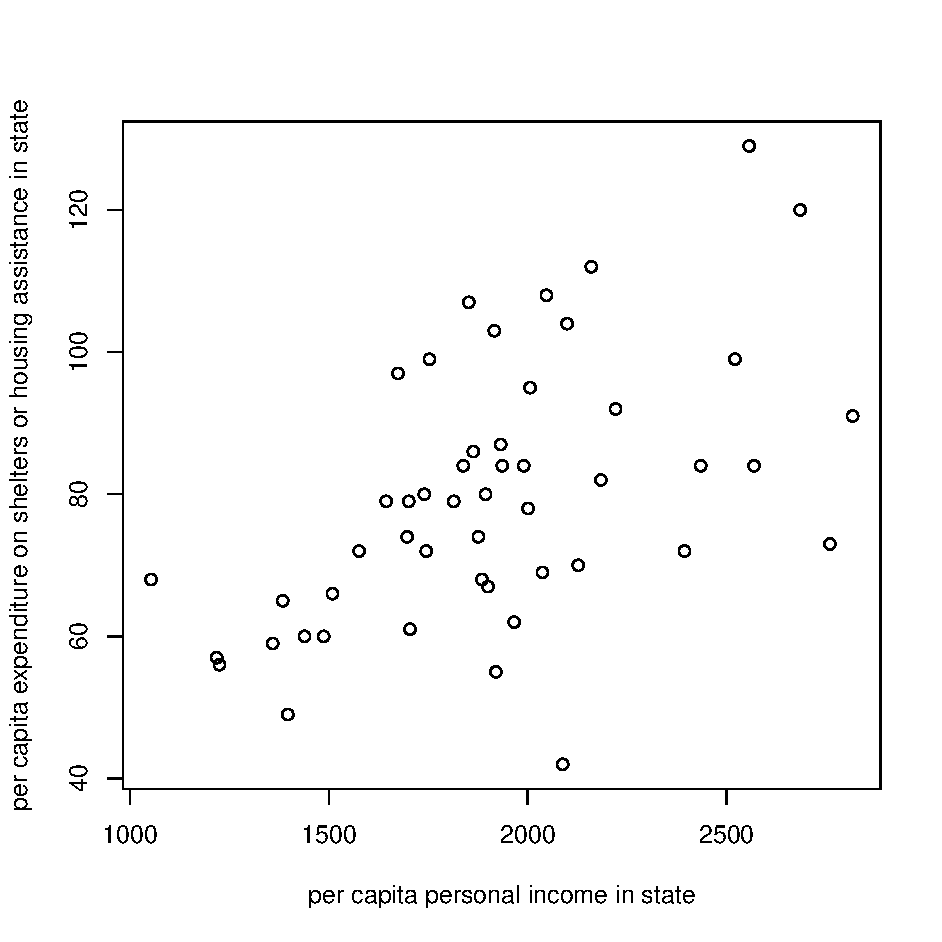
\includegraphics[width=8cm]{X1 Y Graph.pdf}
    \caption{This chart demonstrates that the more personal income in a state the more money that is spent on housing and shelter assistance in a state. Low income is associated with low spending in this area.}
    \label{X1, Y}
\end{figure}

\begin{figure}[htp]
    \centering
    \includegraphics[width=8cm]{X1, X2 Graph.pdf}
    \caption{The highest number of people that are deemed financially insecure in a state are in the 1500 to 2000 dollar mid range of personal income.
}
    \label{X1, X2}
\end{figure}


\begin{figure}[htp]
    \centering
    \includegraphics[width=8cm]{x1 x3 Graph.pdf}
    \caption{We can see that the highest levels of personal income are associated with  the highest number of people living in urban areas.
}
    \label{X1, X3}
\end{figure}

\begin{figure}[htp]
    \centering
    \includegraphics[width=8cm]{Y, X2 Graph.pdf}
    \caption{Lower numbers of residents  deemed financially insecure are associated with lower expenditure on shelter and housing assistance. The higher number of financially insecure individuals in a state is associated with higher spending in relation to housing assistance.
}
    \label{Y, X2}
\end{figure}

\begin{figure}[htp]
    \centering
    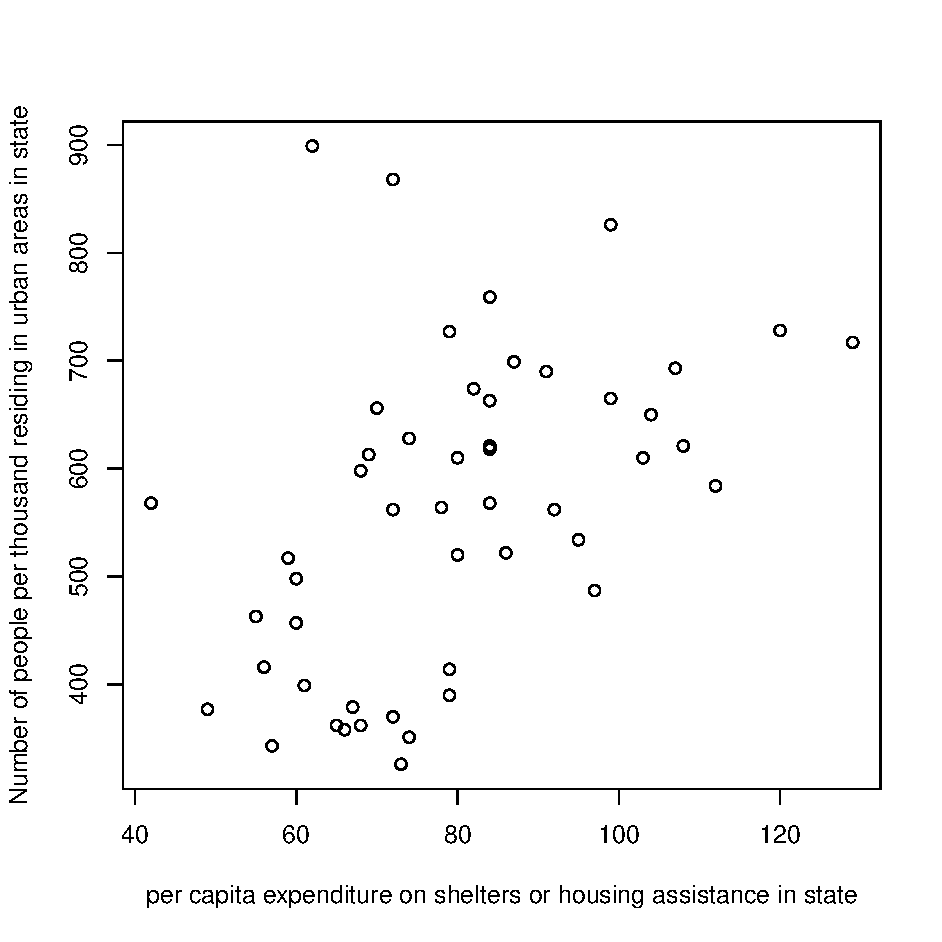
\includegraphics[width=8cm]{Y, X3 Graph.pdf}
    \caption{Low levels of shelter or housing assistance expenditure is associated with lower populations of people residing in urban areas. The more individuals residing in the urban areas of states the higher the expenditure in relation to housing assistance.
}
    \label{Y, X3}
\end{figure}

\begin{figure}[htp]
    \centering
    \includegraphics[width=8cm]{X2, X3 Graph.pdf}
    \caption{We can see here that there is not a strong relationship between these two variables. Lower numbers of individuals in financially insecure states occur both in high and low numbers of individuals living in urban areas.
}
    \label{x2, x3}
\end{figure}



\begin{figure}[htp]
    \centering
    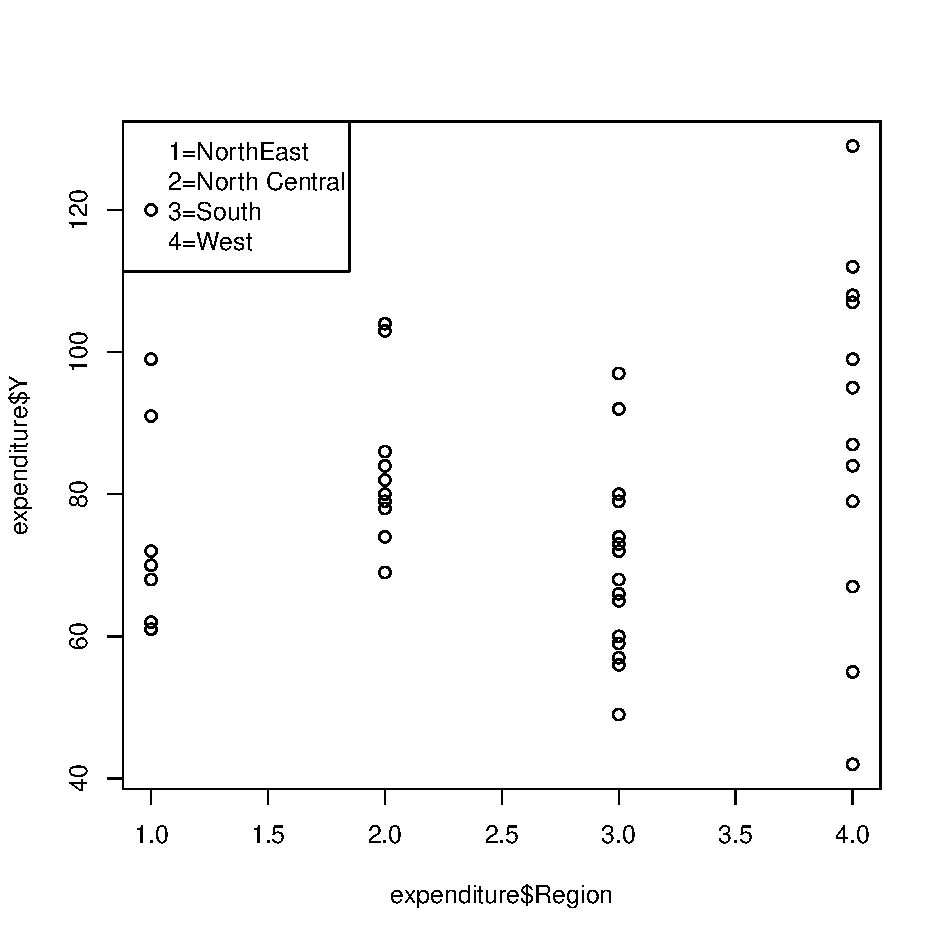
\includegraphics[width=8cm]{Region and Y.pdf}
    \caption{Q2PT2: The west region has the highest expenditure on housing and shelter assistance on average.
}
    \label{Region, Y}
\end{figure}



\begin{figure}[htp]
    \centering
    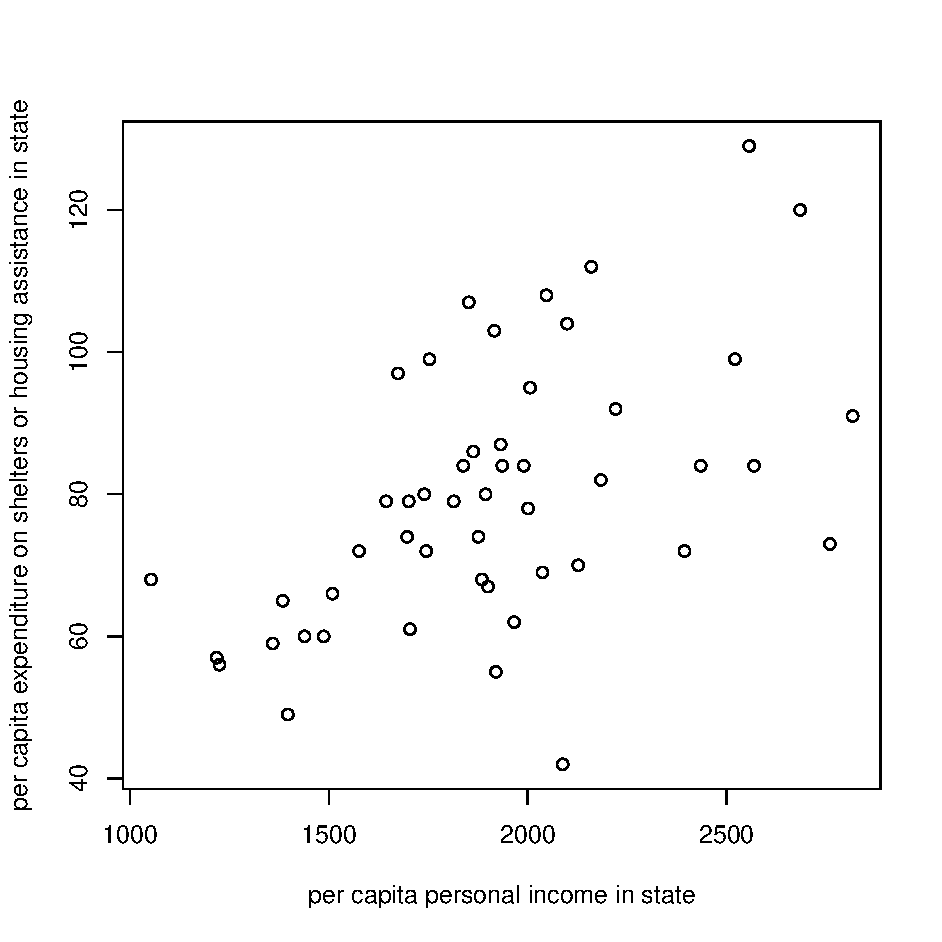
\includegraphics[width=8cm]{X1 Y Graph.pdf}
    \caption{Q2PT3: We can see that higher spending on housing and shelter assistance is generally associated with higher personal income in that state. This is not true for all cases though as we can see the highest personal income values occur in the mid range of expenditure on housing assistance.
}
    \label{X1, Y}
\end{figure}

\begin{figure}[htp]
    \centering
    \includegraphics[width=8cm]{X1, Y and Region.pdf}
    \caption{Here we see the relationship between X1 and Y. Region is represented by color.
}
    \label{x1, y, Region}
\end{figure}
\

\end{document}